% Solution: Tadelis (2013) Exercise 7.9 "The Dean's Dilemma". Input by \solitem.
% New in the 50-item list. Check: check_B_L03.py.
\begin{exsol}{Tadelis Exercise 7.9}{149--150}{Exam}{4}
\asked The dean learns whether he has evidence (probability $\frac12$), then accuses ($A$) or
bounces ($B$); an accused student, who does not know whether there is evidence, confesses ($C$)
or denies ($D$). (a) Game tree; (b) normal-form matrix; (c) Nash equilibria.

\method A move of Nature at the root and information sets for what a player does not observe
(Lecture~3, slides~21--23; Tadelis \S7.1, Def.~7.2, p.~135; Nature as in the Brexit tree, Lecture~4,
slides~5--6). Strategies as plans over information sets (Lecture~3, slide~25), with expected
payoffs over Nature's move in the normal form (Tadelis \S7.2.3, pp.~142--145). Nash equilibria by
dominance, best replies and the principle of indifference (Lecture~3, slides~10--12).

\solution
\textbf{Notation.} Nature draws $e$ (evidence) or $n$ (no evidence), each with probability
$\frac12$. The dean (player~1) observes it. Payoffs $(u_1, u_2)$ = (dean, student):
$B \mapsto (0,0)$; $A,C \mapsto (2,-2)$; $A,D$ with evidence $\mapsto (4,-4)$; $A,D$ without
evidence $\mapsto (-4,4)$. Note that $u_1 + u_2 = 0$ at every leaf: the game is zero-sum.

\textbf{(a) Tree.} The student's two nodes (after $eA$ and after $nA$) form one information set: he
knows he was accused, not whether there is evidence.
\begin{center}
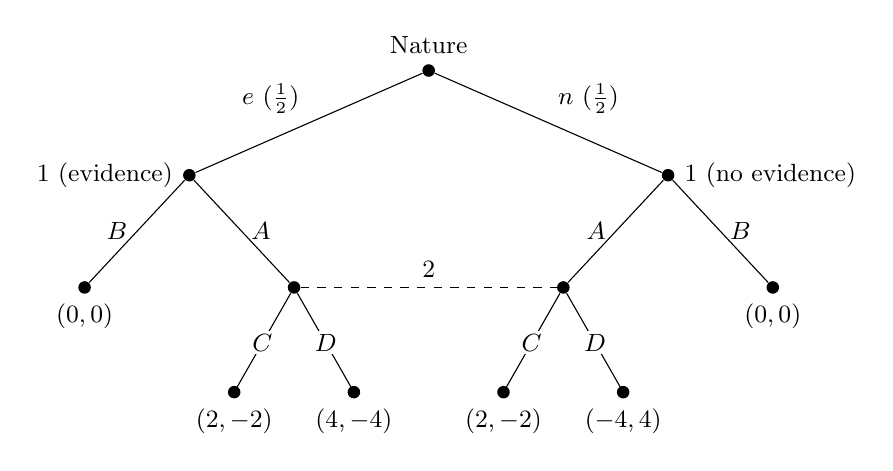
\begin{tikzpicture}[scale=0.95,dot/.style={circle,fill,inner sep=1.6pt},
  every node/.style={font=\small}]
  \node[dot,label=above:{Nature}] (r) at (0,0) {};
  \node[dot,label=left:{1 (evidence)}] (e) at (-3.2,-1.4) {};
  \node[dot,label=right:{1 (no evidence)}] (n) at (3.2,-1.4) {};
  \draw (r) -- node[above left] {$e$ ($\frac12$)} (e);
  \draw (r) -- node[above right] {$n$ ($\frac12$)} (n);
  \node[dot,label=below:{$(0,0)$}] (eb) at (-4.6,-2.9) {};
  \node[dot] (ea) at (-1.8,-2.9) {};
  \node[dot] (na) at (1.8,-2.9) {};
  \node[dot,label=below:{$(0,0)$}] (nb) at (4.6,-2.9) {};
  \draw (e) -- node[left] {$B$} (eb);
  \draw (e) -- node[right] {$A$} (ea);
  \draw (n) -- node[left] {$A$} (na);
  \draw (n) -- node[right] {$B$} (nb);
  \draw[dashed] (ea) -- node[above] {2} (na);
  \foreach \xx/\p/\lab/\pay in {-2.6/ea/$C$/{$(2,-2)$}, -1.0/ea/$D$/{$(4,-4)$},
                               1.0/na/$C$/{$(2,-2)$}, 2.6/na/$D$/{$(-4,4)$}} {
    \node[dot,label=below:{\pay}] at (\xx,-4.3) {};
    \draw (\p) -- node[fill=white,inner sep=1pt] {\lab} (\xx,-4.3);
  }
\end{tikzpicture}
\end{center}

\textbf{(b) Normal form.} The dean has two information sets, so a strategy is a pair
(action with evidence, action without): $S_1 = \{AA, AB, BA, BB\}$; $S_2 = \{C, D\}$. Each cell
is $\frac12 \times$(payoff after $e$) $+ \frac12 \times$(payoff after $n$). For example,
$u(AB, D) = \frac12(4,-4) + \frac12(0,0) = (2,-2)$ and $u(AA, D) = \frac12(4,-4) + \frac12(-4,4) =
(0,0)$.
\begin{center}
\begin{tabular}{r|c|c|}
\multicolumn{1}{r}{} & \multicolumn{1}{c}{$C$} & \multicolumn{1}{c}{$D$}\\ \cline{2-3}
$AA$ & $\br{2},\ -2$ & $0,\ \br{0}$ \\ \cline{2-3}
$AB$ & $1,\ \br{-1}$ & $\br{2},\ -2$ \\ \cline{2-3}
$BA$ & $1,\ -1$ & $-2,\ \br{2}$ \\ \cline{2-3}
$BB$ & $0,\ \br{0}$ & $0,\ \br{0}$ \\ \cline{2-3}
\end{tabular}
\end{center}

\textbf{(c) Nash equilibria.}

\emph{Step 1: no pure equilibrium.} No cell has both payoffs underlined: against $C$ the dean
plays $AA$, against which the student denies; against $D$ the dean plays $AB$, against which the
student confesses. The best replies cycle.

\emph{Step 2: dominated strategies.} $BA$ is strictly dominated by $AA$ ($2 > 1$, $0 > -2$):
accusing only when there is no evidence is never sensible. $BB$ is strictly dominated by $AB$
($1 > 0$, $2 > 0$). So in any equilibrium the dean accuses whenever he has evidence and mixes only
between $AA$ and $AB$, i.e.\ over what he does \emph{without} evidence.

\emph{Step 3: indifference.} Let $q = \Pr_2(C)$ and $p = \Pr_1(AA)$ (with $1-p$ on $AB$). The dean
is indifferent when
\begin{equation}
  u_1(AA) = 2q \;=\; q + 2(1-q) = u_1(AB) \;\Rightarrow\; 2q = 2 - q \;\Rightarrow\; q = \tfrac23 ,
  \label{eq:tadelis-7-9-q}
\end{equation}
and the student is indifferent when
\begin{equation}
  u_2(C) = -2p - (1-p) \;=\; 0\cdot p - 2(1-p) = u_2(D) \;\Rightarrow\; -1 - p = -2 + 2p
  \;\Rightarrow\; p = \tfrac13 . \label{eq:tadelis-7-9-p}
\end{equation}
At $q = \frac23$ the dean's payoffs are $AA, AB: \frac43$, $BA: 3q - 2 = 0$, $BB: 0$, so mixing
over $AA$ and $AB$ is optimal. The unique Nash equilibrium is
\[
  \sigma_1^* = \tfrac13\,AA + \tfrac23\,AB, \qquad \sigma_2^* = \tfrac23\,C + \tfrac13\,D,
  \qquad (u_1, u_2) = \bigl(\tfrac43,\ -\tfrac43\bigr).
\]
\emph{Uniqueness.} For $q < \frac23$ only $AB$ is a best reply and the student would then confess
($-1 > -2$), so $q = 1$; for $q > \frac23$ only $AA$ is a best reply and the student would deny
($0 > -2$), so $q = 0$; at $q = \frac23$ only $p = \frac13$ keeps the student indifferent.

\emph{Behavioral reading.} With evidence the dean always accuses; without evidence he accuses
(bluffs) with probability $\frac13$. An accused student therefore faces evidence with probability
$\frac{1/2}{1/2 + 1/2\cdot1/3} = \frac34$, and at that belief $C$ and $D$ both give $-2$ (the check:
$\frac34(-4) + \frac14(4) = -2$).

\interp The dean must bluff sometimes: if he accused only with evidence, every accusation would
reveal evidence and the student would confess, which in turn makes accusing without evidence
profitable. The equilibrium bluffing rate keeps the student exactly indifferent. Because the game
is zero-sum, $\frac43$ is its value: the dean cannot guarantee more, the student cannot hold him
to less. The structure (Nature, a privately informed first mover, a responder who sees only the
action) is the one Lecture~4 used for the Brexit negotiation, and it is the bridge to games of
incomplete information later in the course.

\verify \texttt{check\_B\_L03.py} builds the matrix from the tree with exact fractions (it equals the
one above), checks the zero-sum property and that there is no pure equilibrium, scans $q$ on a grid
of step $\frac1{300}$ (an equilibrium exists only at $q = \frac23$), verifies
$(\frac13 AA + \frac23 AB,\ \frac23 C + \frac13 D)$ with the exact Nash test, and solves
\eqref{eq:tadelis-7-9-p} with sympy. Output line: \texttt{tadelis-7-9: unique NE dean 1/3 AA + 2/3
AB, student C w.p. 2/3; value 4/3}. Tadelis prints no answer.

\mistakes
\begin{itemize}
  \item Giving the dean only two strategies ($A$, $B$): he chooses after observing Nature, so a
  strategy is a pair of actions.
  \item Drawing the student's two nodes as separate information sets: then he would know whether
  there is evidence, and the game would change completely.
  \item Using payoffs conditional on one state in the matrix instead of the $\frac12$--$\frac12$
  expectation.
\end{itemize}

\answer{(a) Tree above, with the student's nodes in one information set. (b) Matrix above, rows
$AA, AB, BA, BB$ (action with evidence, without). (c) No pure equilibrium; unique Nash equilibrium
$(\frac13 AA + \frac23 AB,\ \frac23 C + \frac13 D)$: the dean always accuses with evidence and
bluffs w.p.\ $\frac13$ without it; the student confesses w.p.\ $\frac23$; payoffs
$(\frac43, -\frac43)$.}
\end{exsol}
